\documentclass[14pt]{beamer}
\mode<presentation>
\usetheme{Warsaw}
%\usetheme{Marburg}
\usecolortheme{seahorse}
%\usefonttheme{serif}
\usepackage{url}
\usepackage{fancyvrb}
\usepackage{graphicx}
\usepackage{subfigure}
\usepackage{color}

\definecolor{Highlight}{RGB}{255,0,0}

\author{HU, Pili}
\title{Adaptive Video Streaming}
\institute{\url{http://personal.ie.cuhk.edu.hk/~hpl011/}}
\subtitle{A Survey and Case Study}
%\institution{MobiTec/IE/CUHK}

\begin{document}

\begin{frame}
\titlepage
\end{frame}

%\frame<100>[label=contents]{
%\frametitle{Contents}
%\begin{itemize}
%\item Youtube
%	\begin{itemize}
%		\item<alert@1> Environment
%		\item<alert@2> Video Information
%		\item<alert@3> Observation
%		\item<alert@4> Conclusion
%		\item<alert@5> Bypass Flow Control
%	\end{itemize}
%\item Douban.fm
%	\begin{itemize}
%		\item<alert@6> Conclusion
%	\end{itemize}
%\end{itemize}
%}

%\againframe<1>{contents}

\begin{frame}
\frametitle{Landscape of Adaptive Video Streaming}
	\begin{itemize}
		\item MDC, MLC. 
		\item Multicast(1996), Unicast(2001), P2P(still chaos)
		\item ASTRI:
			\begin{itemize}
				\item Current Version: multi channel layered VoD 
				(real deployment)
				\item Simulation platform: single channel fixed initial layer
				VoD
				(trial version, [wen, 2010])
			\end{itemize}
	\end{itemize}
\end{frame}

\begin{frame}
\frametitle{Landscape of Adaptive Video Streaming}
\framesubtitle{Version Trees}
\begin{figure}
	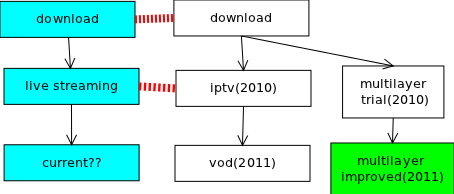
\includegraphics[width=0.6\textwidth]{../fig/version_tree.png}
	\caption{Version Tree of Real and Simulation}
\end{figure}
\begin{itemize}
	\item Blue: Real deployment
	\item While: Simulation platform 
	\item Green: This work  
	\item Red dash: Equivalency
\end{itemize}
\end{frame}

\begin{frame}
\frametitle{Performance Benchmark}
\framesubtitle{runtime v.s. \# of core}
\begin{figure}
	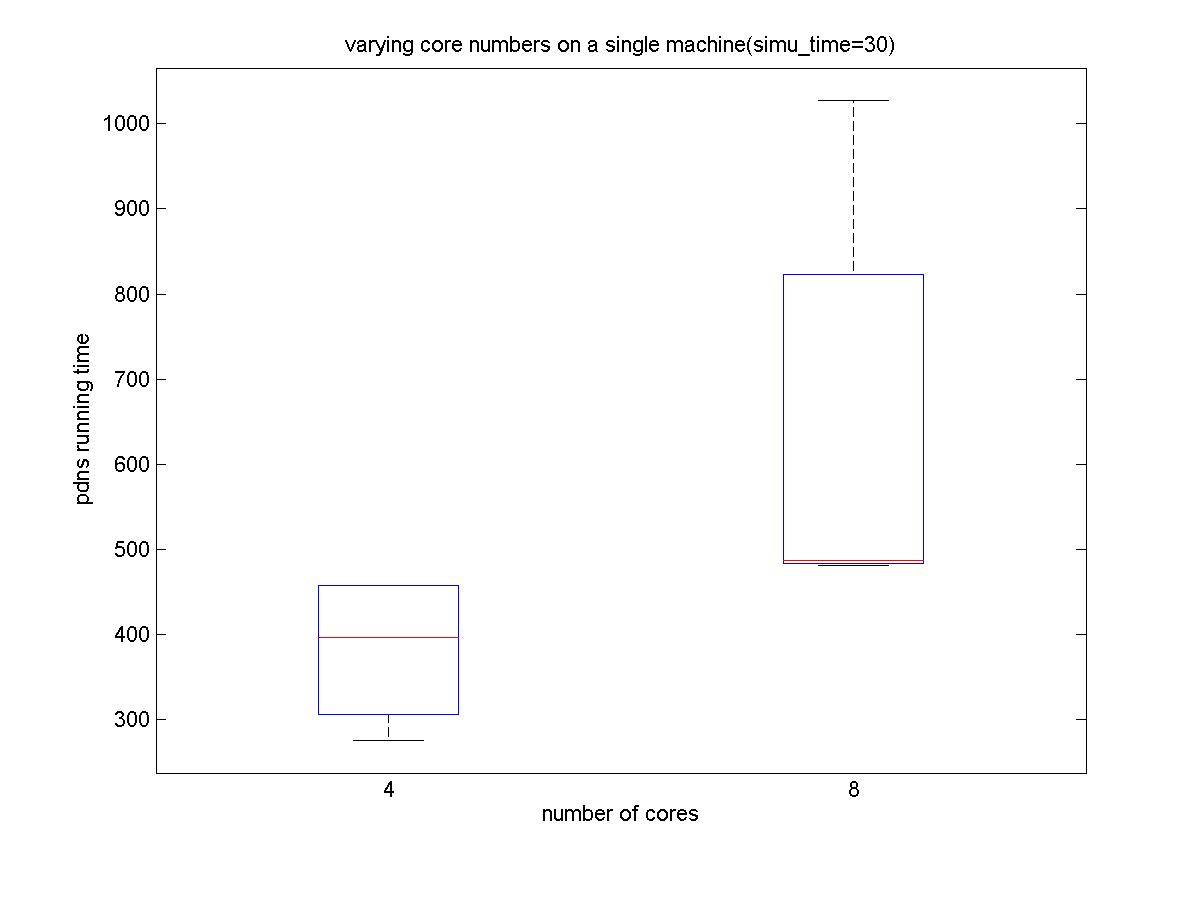
\includegraphics[width=0.8\textwidth]{../fig/runtime_vs_core.jpg}
\end{figure}
\end{frame}

\begin{frame}
\frametitle{Performance Benchmark}
\framesubtitle{runtime v.s. simulation time}
\begin{figure}
	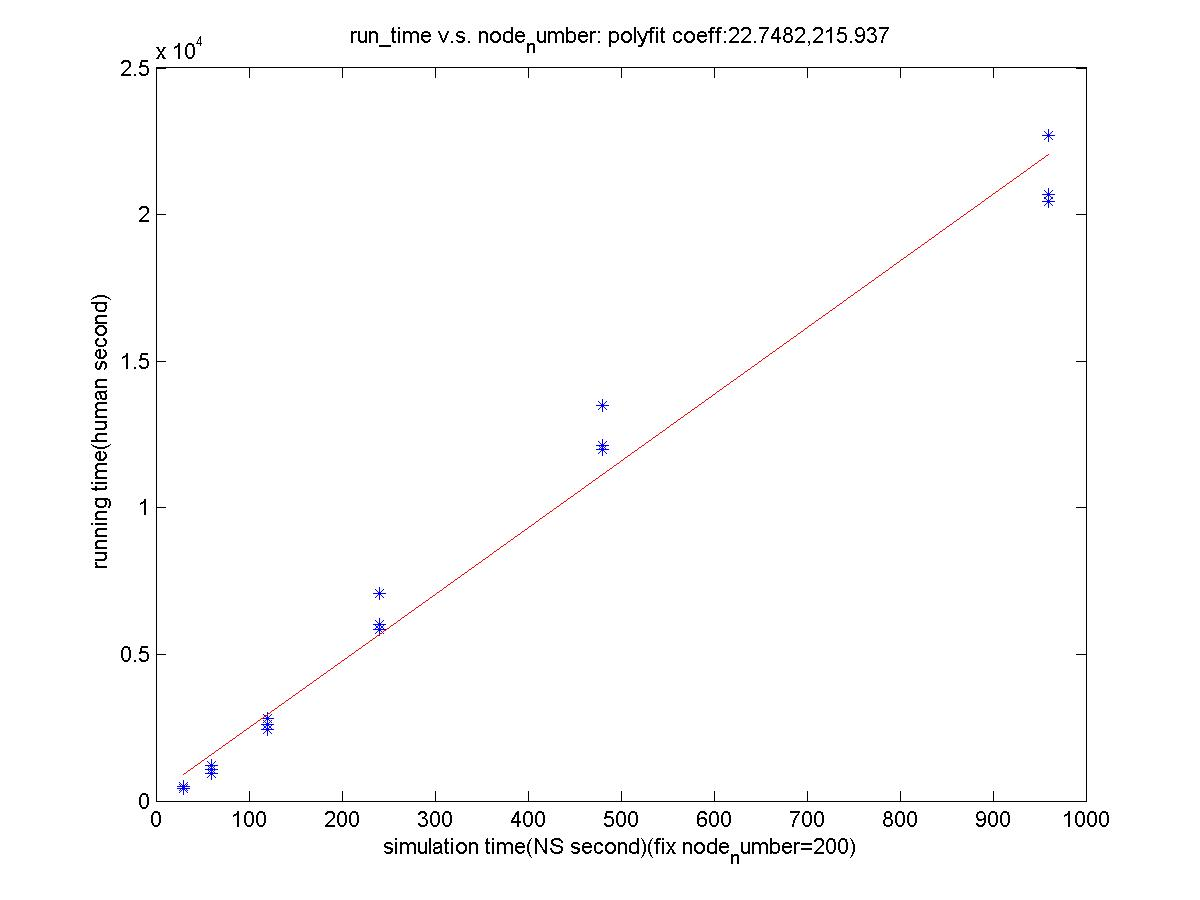
\includegraphics[width=0.8\textwidth]{../fig/runtime_vs_nodenum.jpg}
\end{figure}
\end{frame}

\begin{frame}
\frametitle{Performance Benchmark}
\framesubtitle{runtime v.s. \# of nodes}
\begin{figure}
	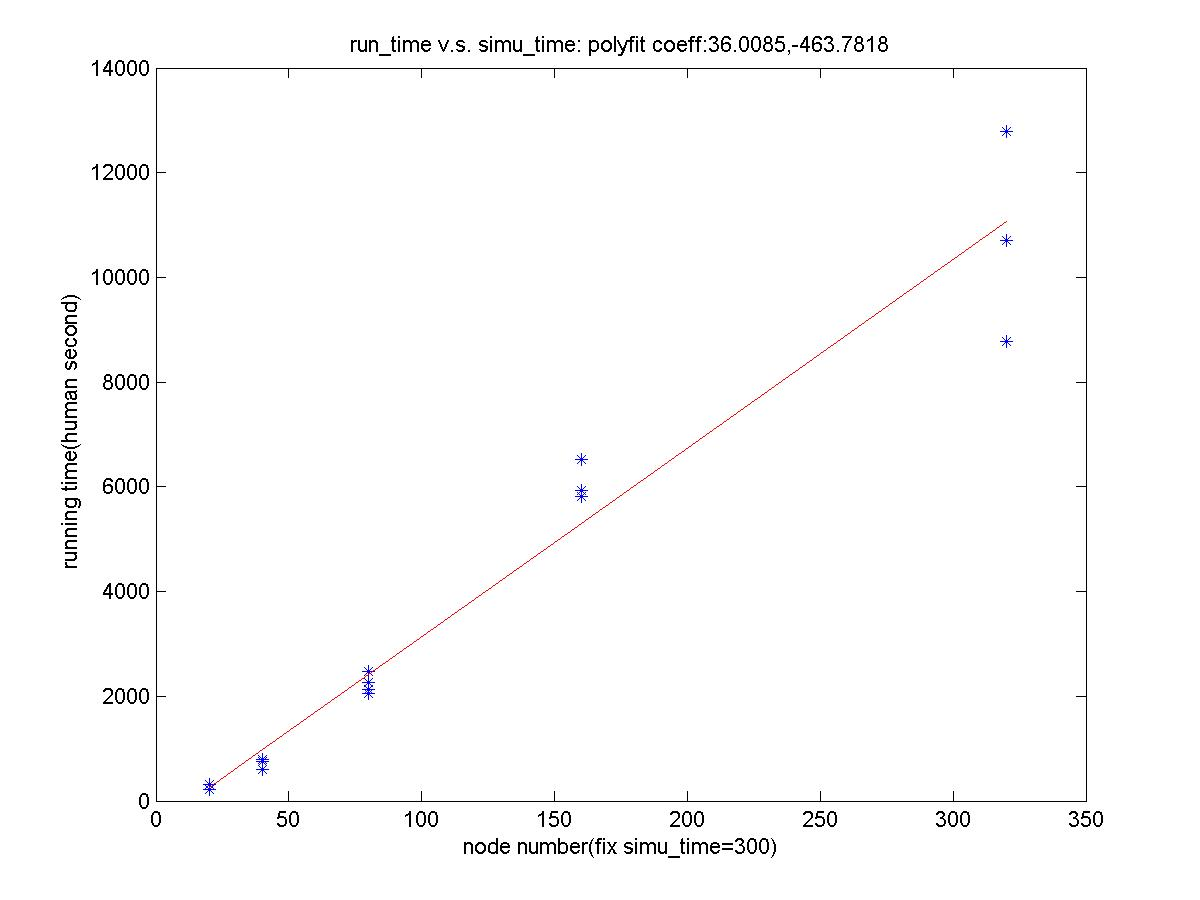
\includegraphics[width=0.8\textwidth]{../fig/runtime_vs_simutime.jpg}
\end{figure}
\end{frame}

\begin{frame}
\frametitle{Simulation Confuguration}
\framesubtitle{Basic Settings}
\begin{itemize}
	\item Number of Nodes: 160
	\item Simulation Time: 300 (NS seconds)
\end{itemize}
\end{frame}

\begin{frame}
\frametitle{Simulation Confuguration}
\framesubtitle{Topology and Capacity}
Wen Zheng's configuration:
\begin{itemize}
	\item Star like, 4 subnet. 
	\item Subnet parameters:
		\begin{itemize}
			\item Subnet1: down:10Mb; up:10Mb. 
			\item Subnet1: down:3Mb; up:0.5Mb. 
			\item Subnet1: down:3Mb; up:0.5Mb. 
			\item Subnet1: down:3Mb; up:0.5Mb. 
		\end{itemize}
\end{itemize}
\end{frame}

\begin{frame}
\frametitle{Simulation Confuguration}
\framesubtitle{Layers}
\begin{itemize}
	\item 3 Layers. Conform to [wang,2011] QoE study.  
	\item Layer parameters:
		\begin{itemize}
			\item Layer1: 256Kbit. (per piece) 
			\item Layer2: 256Kbit. (per piece) 
			\item Layer3: 512Kbit. (per piece) 
		\end{itemize}
\end{itemize}
Cumulative layer piece size is: 256, 512, 1024 (Kbit). 
\end{frame}

\begin{frame}
\frametitle{QoE Model Adopted}
[wang, 2011], B-D tradeoff, continuous version. 
\begin{equation}
	MOS = c_1 \times d + \alpha \times (1 - e^{-b \times \lambda}) + c_2
\end{equation}
\begin{figure}
	\subfigure[3D]{
	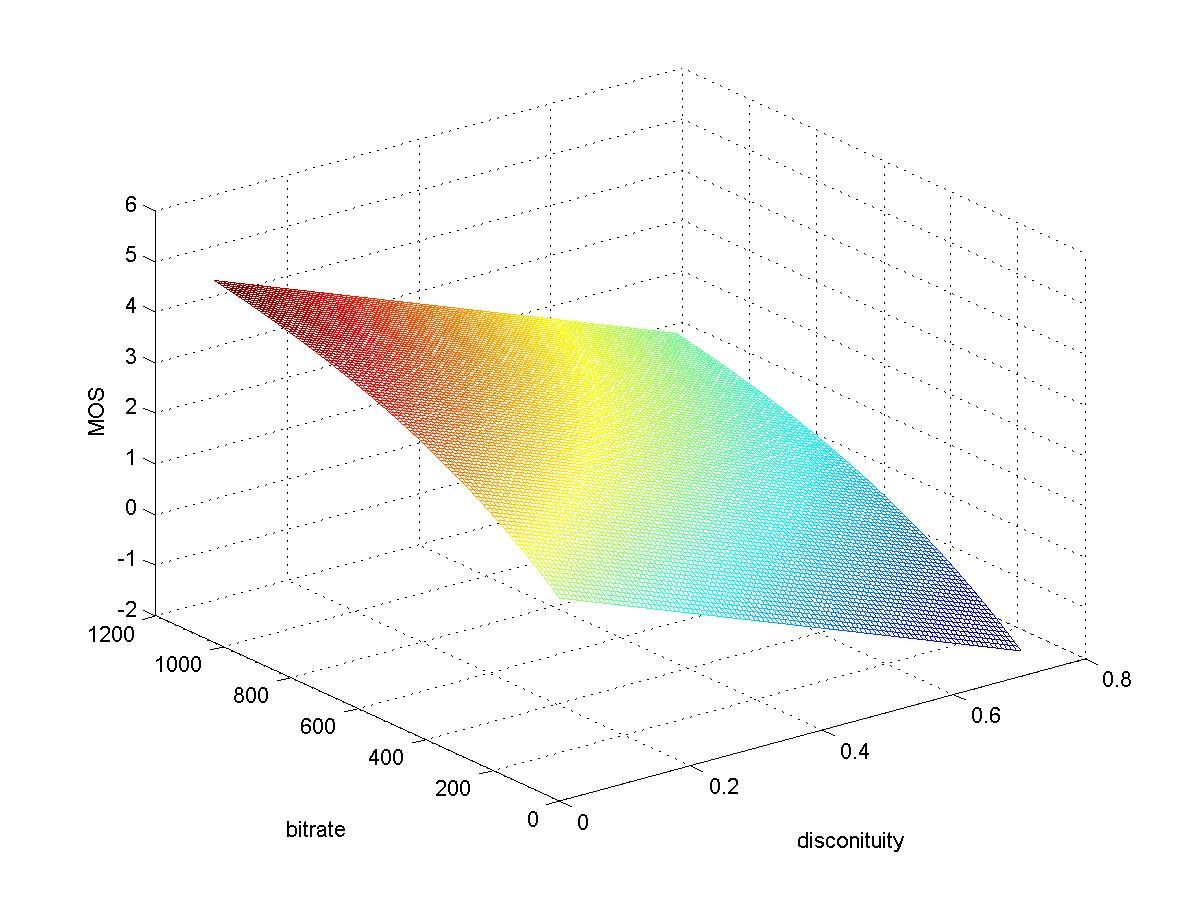
\includegraphics[width=0.45\textwidth]{../fig/bd_3d.jpg}
	}
	\subfigure[contour]{
	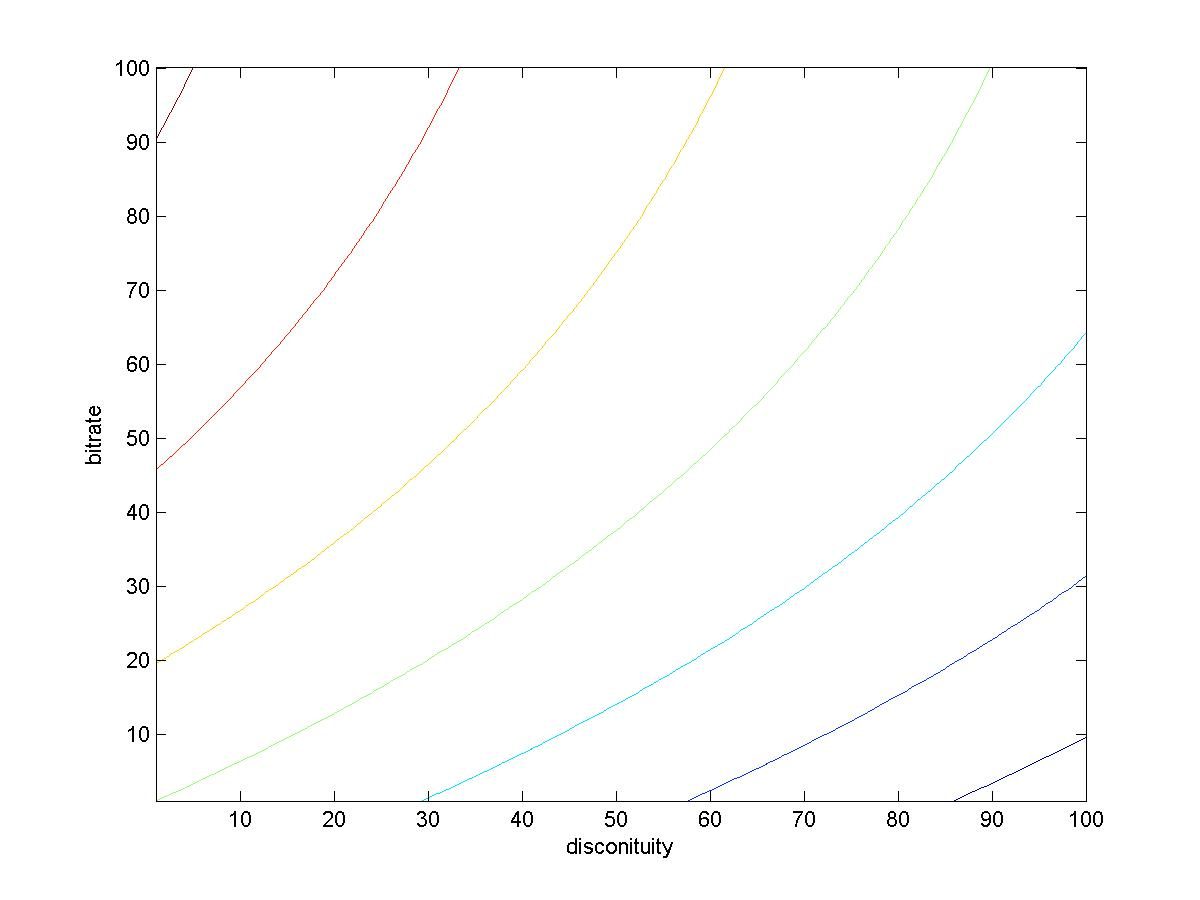
\includegraphics[width=0.45\textwidth]{../fig/bd_contour.jpg}
	}
	\caption{Conclusion, QoE and Performance}
\end{figure}
\end{frame}

\begin{frame}
\frametitle{Baseline Test}
\framesubtitle{QoE v.s. simulation time}
\begin{figure}
	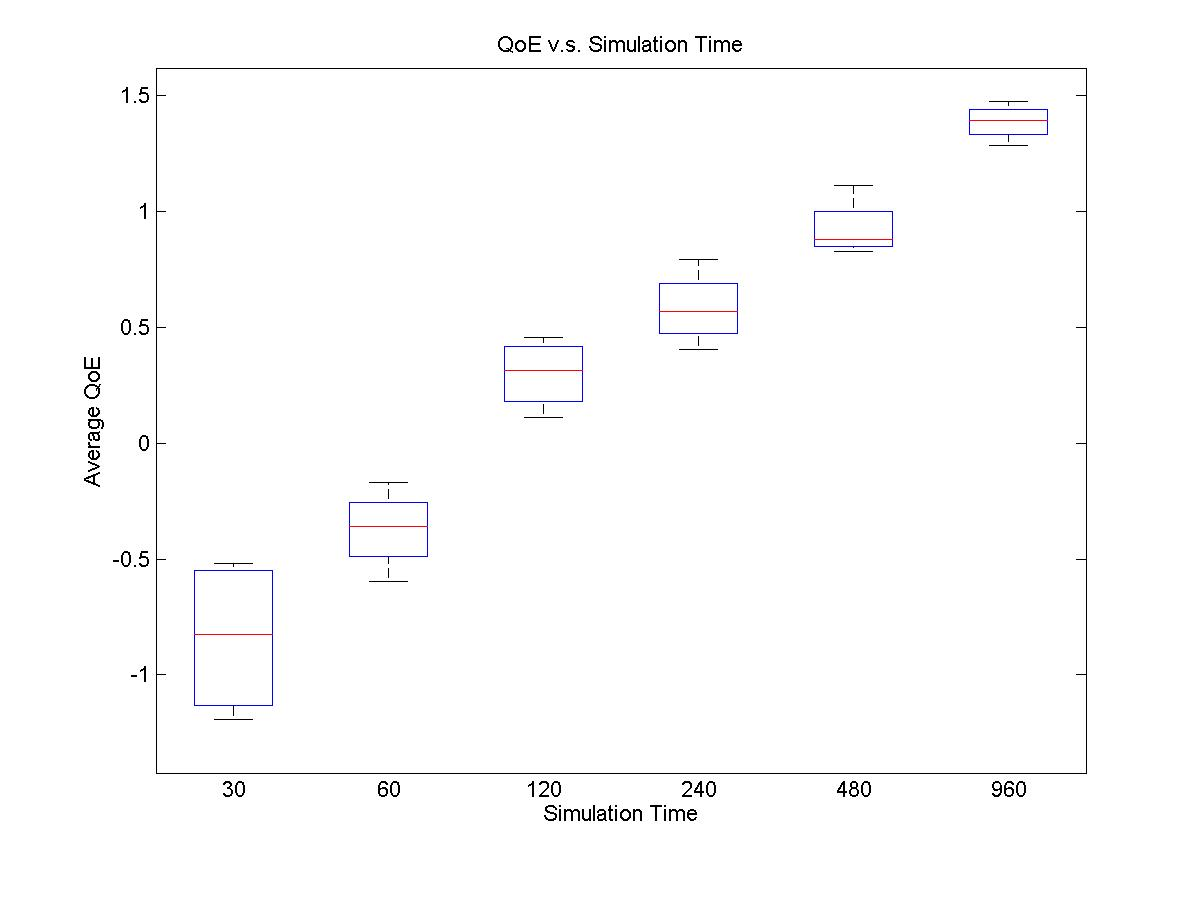
\includegraphics[width=0.8\textwidth]{../fig/simutime_qoe.jpg}
\end{figure}
\end{frame}

\begin{frame}
\frametitle{Baseline Test}
\framesubtitle{QoE(nonneg) v.s. simulation time}
\begin{figure}
	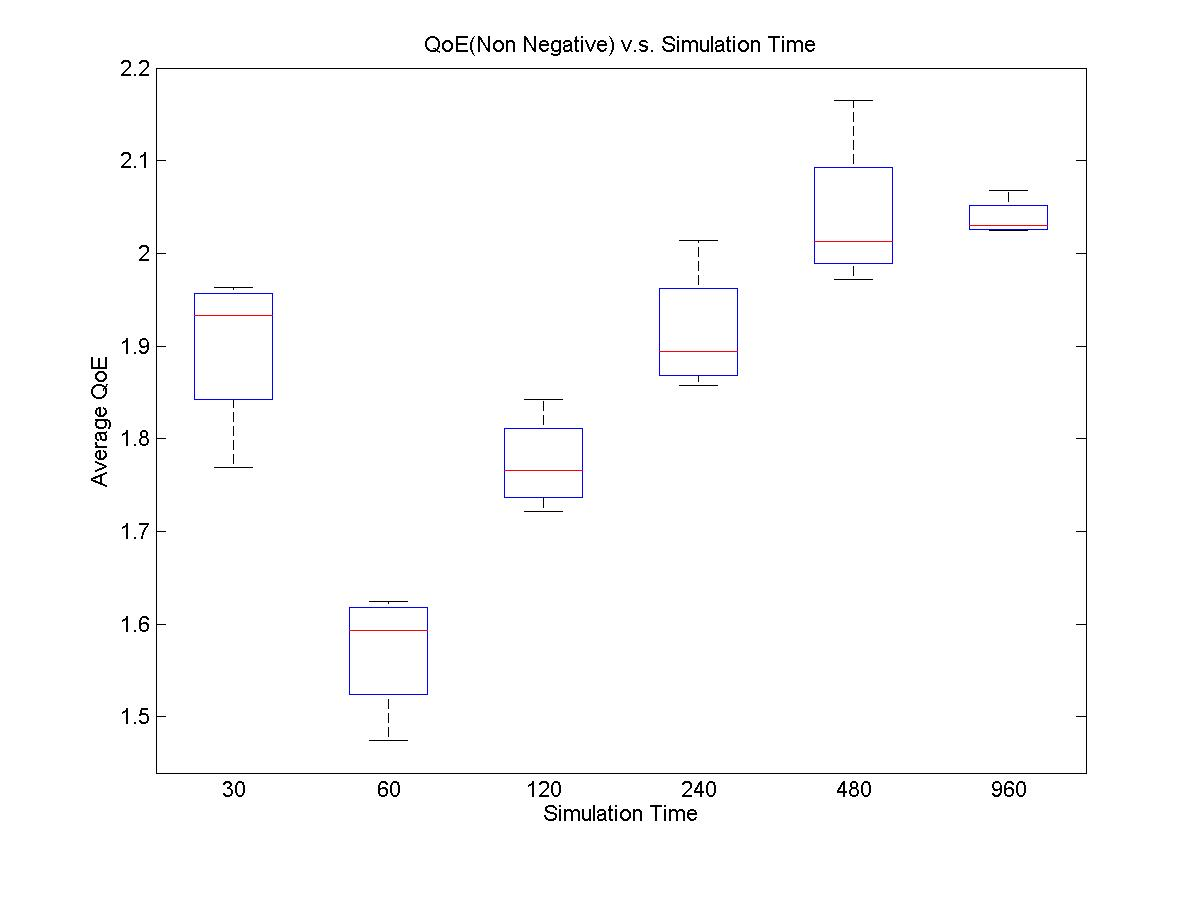
\includegraphics[width=0.8\textwidth]{../fig/simutime_qoe_nonneg.jpg}
\end{figure}
\end{frame}

\begin{frame}
\frametitle{Baseline Test: A Sample Run}
\framesubtitle{Configuration}
\begin{itemize}
      \item     $'count\_mr' => 3749$
      \item     $'count\_mr\_nonneg' => 2601$
      \item     $'avg\_qoe' => '0.871540677419684'$
      \item     $'avg\_qoe\_nonneg' => '2.01996612593628'$
      \item     $'node\_num' => '160'$
      \item     $'simu\_time' => '480'$
      \item     $'core\_num' => '4'$
      \item     $'task\_duration' => 8399$
      \item     $'pdns\_duration' => 8302$
\end{itemize}
\end{frame}

\begin{frame}
\frametitle{Baseline Test: A Sample Run}
\framesubtitle{QoE v.s. time slot}
\begin{figure}
	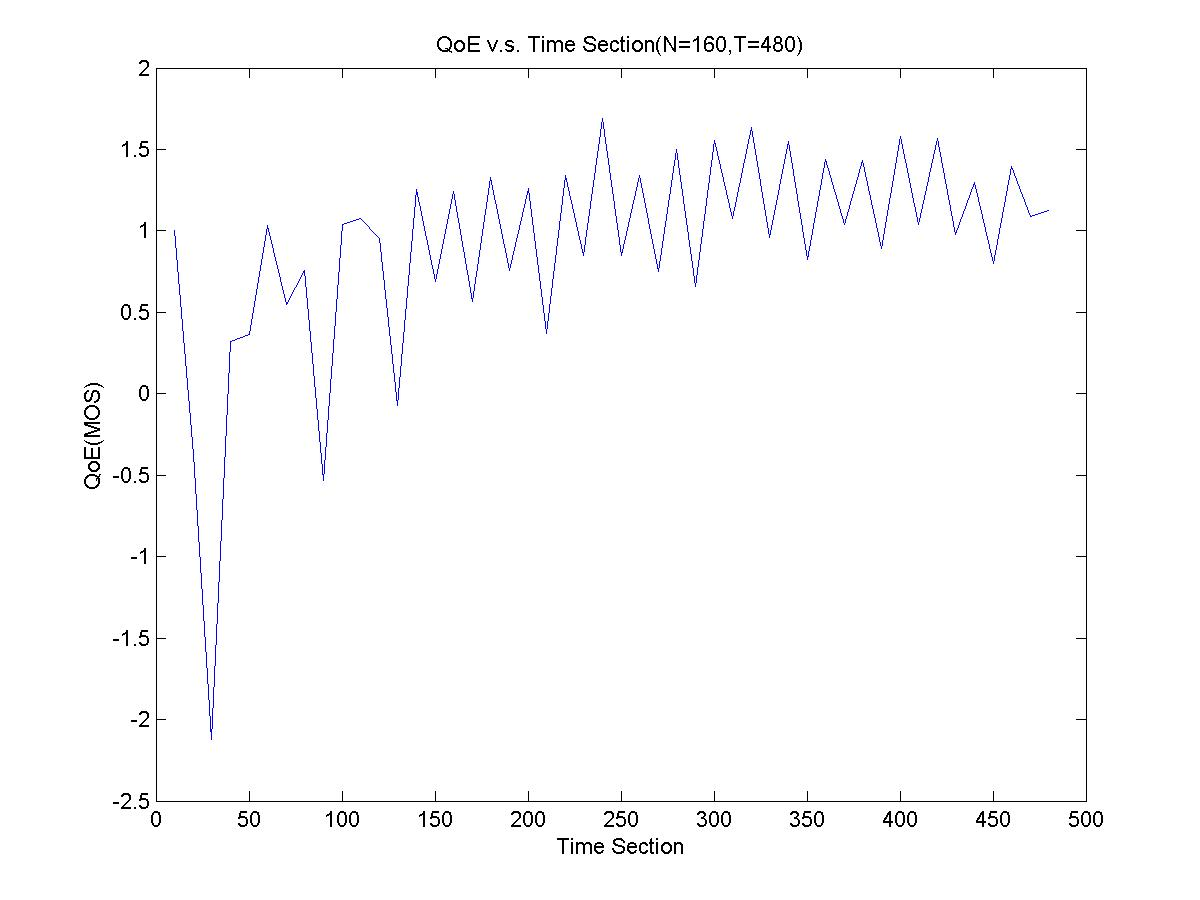
\includegraphics[width=0.6\textwidth]{../fig/time_qoe.jpg}
\end{figure}
Observations:
\begin{itemize}
	\item System bootstraping stage. 
	\item Steady after about 250 seconds. 
\end{itemize}
\end{frame}

\begin{frame}
\frametitle{Baseline Test: A Sample Run}
\framesubtitle{histogram of 3749 QoE reports}
\begin{figure}
	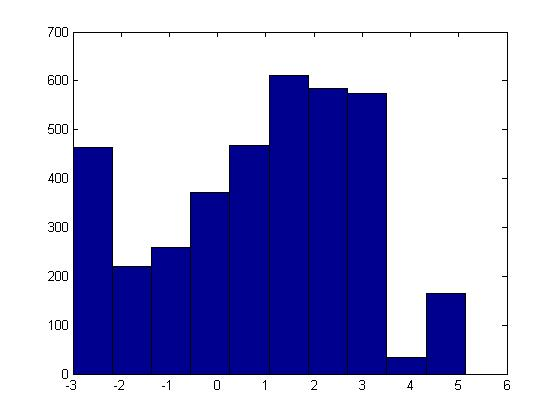
\includegraphics[width=0.7\textwidth]{../fig/qoe_hist.jpg}
\end{figure}
\end{frame}


\begin{frame}
\frametitle{Version2: Unified Architecture}
\framesubtitle{original framework}
\begin{figure}
	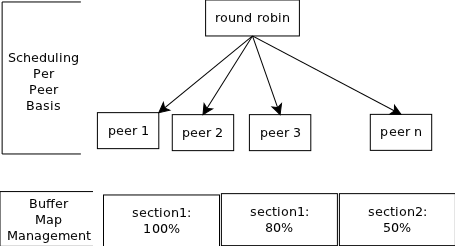
\includegraphics[width=0.7\textwidth]{../fig/arch_orig.png}
	\caption{Original Architecture}
\end{figure}
\end{frame}

\begin{frame}
\frametitle{Version2: Unified Architecture}
\framesubtitle{unified framework}
\begin{figure}
	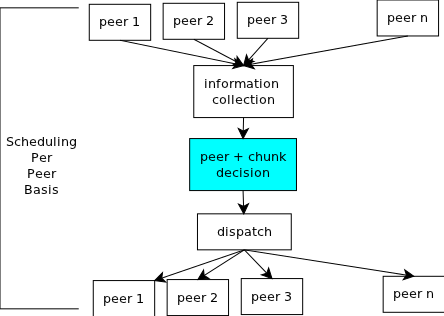
\includegraphics[width=0.7\textwidth]{../fig/arch_improved.png}
	\caption{Improved Architecture}
\end{figure}
\end{frame}

\begin{frame}
\frametitle{Version2: Unified Architecture}
\framesubtitle{PALS like strategy}
\begin{figure}
	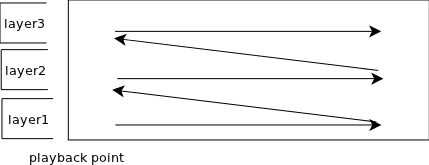
\includegraphics[width=0.7\textwidth]{../fig/pals_like.png}
	\caption{Improved Architecture}
\end{figure}
Effect:
\begin{itemize}
	\item QoE: 0.7 $\rightarrow$ 3.3
\end{itemize}
\end{frame}

\begin{frame}
\frametitle{Version3: Priority Based}
\framesubtitle{framework}
\begin{table}
\caption{A Sample Priority Table with Window Size = 5}
	\begin{tabular}{|c|ccccc|}
	\hline
	 & t1 & t2 & t3 & t4 & t5 \\
	 \hline
	layer3 & 11 & 12 & 13 & 14 & 15 \\
	layer2 & 6 & 7 & 8 & 9 & 10 \\
	layer1 & 1 & 2 & 3 & 4 & 5 \\
	\hline
	\end{tabular}
\end{table}

Result:
\begin{itemize}
	\item QoE: nearly the same. 
	\item Performance: decrease slightly. 
\end{itemize}
\end{frame}


\begin{frame}
\frametitle{Version4: Scalable Window}
\framesubtitle{Reason}
Reason:
\begin{itemize}
	\item From trace, many powerful peeers can get full 3 layers
	in the whole window. 
	\item Give them a chance to download more, and their data
	far from playback pointer can server others. 
\end{itemize}
\begin{table}
\caption{A Sample Priority Table with Window Size = 5+5}
	\begin{tabular}{|c|ccccc|c|}
	\hline
	 & t1 & t2 & t3 & t4 & t5 & t6-t10 \\
	 \hline
	layer3 & 11 & 12 & 13 & 14 & 15 & ...\\
	layer2 & 6 & 7 & 8 & 9 & 10 & ... \\
	layer1 & 1 & 2 & 3 & 4 & 5  & ...\\
	\hline
	\end{tabular}
\end{table}
\end{frame}

\begin{frame}
\frametitle{Version4: Scalable Window}
\framesubtitle{Framework}
\begin{table}
\caption{A Sample Priority Table with Window Size = 5+5}
	\begin{tabular}{|c|ccccc|c|}
	\hline
	 & t1 & t2 & t3 & t4 & t5 & t6-t10 \\
	 \hline
	layer3 & 11 & 12 & 13 & 14 & 15 & ...\\
	layer2 & 6 & 7 & 8 & 9 & 10 & ... \\
	layer1 & 1 & 2 & 3 & 4 & 5  & ...\\
	\hline
	\end{tabular}
\end{table}
Result:
\begin{itemize}
	\item QoE: nearly the same. 
	\item Performance: decrease drastically. 
\end{itemize}
\end{frame}


\begin{frame}
\frametitle{Version5: Performance Optimization}
\framesubtitle{running profile}
\begin{figure}
	\subfigure{
	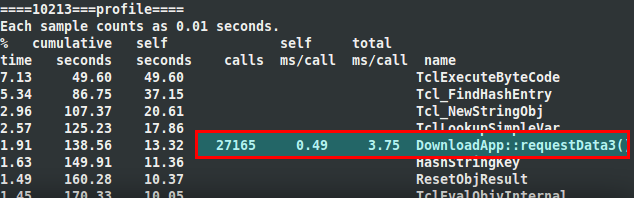
\includegraphics[width=0.6\textwidth]{../fig/gprof1.png}
	} \\
	\subfigure{
	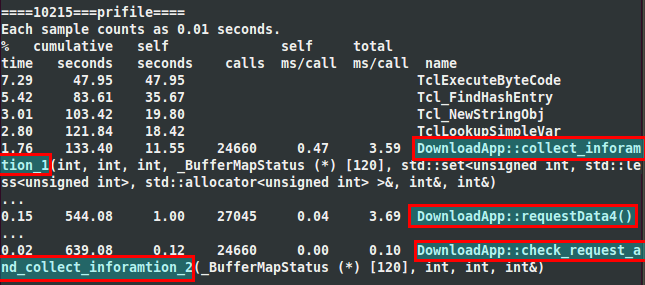
\includegraphics[width=0.6\textwidth]{../fig/gprof2.png}
	}
	\caption{GNU Profile, Output}
\end{figure}
\end{frame}

\begin{frame}
\frametitle{Version5: Performance Optimization}
\framesubtitle{result}
Result:
\begin{figure}
	\item QoE: nearly the same. 
	\item Performance: 4.5h $\rightarrow$ 3.5h. 
\end{figure}
\end{frame}

\begin{frame}
\frametitle{Version6: Random Second Window Section}
\framesubtitle{strategy}
Result:
\begin{itemize}
	\item QoE: worse. 
	\item Performance: worse. 
\end{itemize}
\end{frame}

\begin{frame}
\frametitle{Conclusion}
\framesubtitle{6 big versions comparison}
\begin{figure}
	\subfigure[qoe]{
	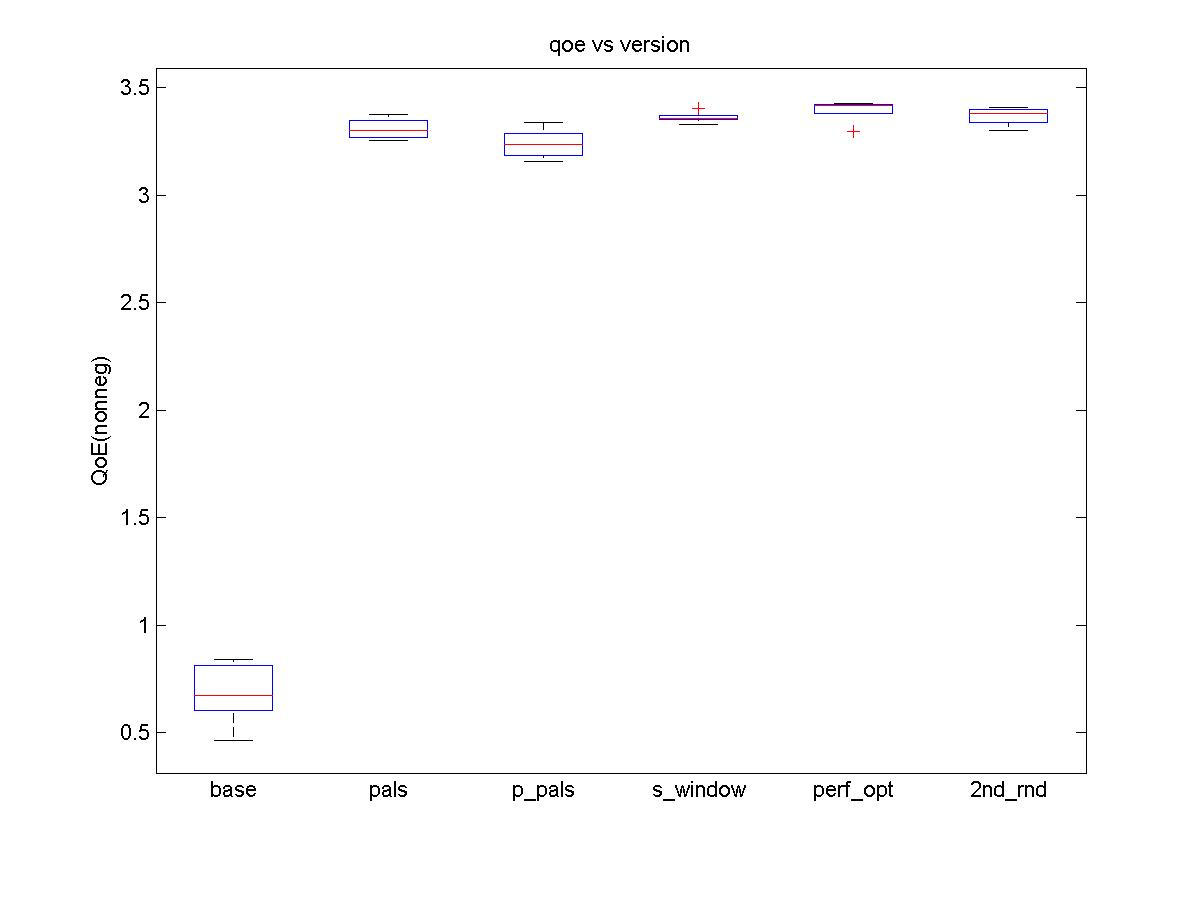
\includegraphics[width=0.45\textwidth]{../fig/con_qoe_version_all.jpg}
	}
	\subfigure[time]{
	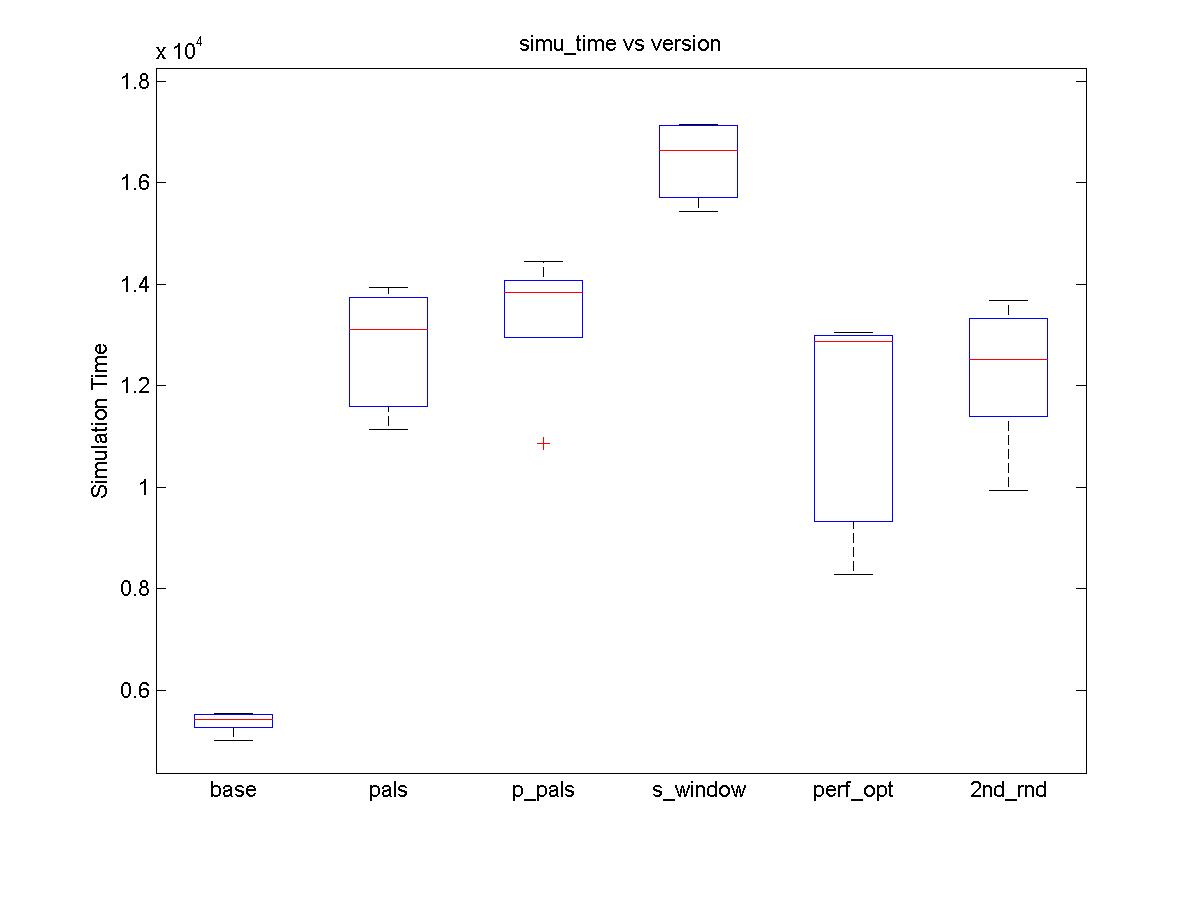
\includegraphics[width=0.45\textwidth]{../fig/con_time_version_all.jpg}
	}
	\caption{Conclusion, QoE and Performance}
\end{figure}
\end{frame}

\begin{frame}
\frametitle{Conclusion}
\framesubtitle{5 enhanced versions comparision(detail)}
\begin{figure}
	\subfigure[qoe]{
	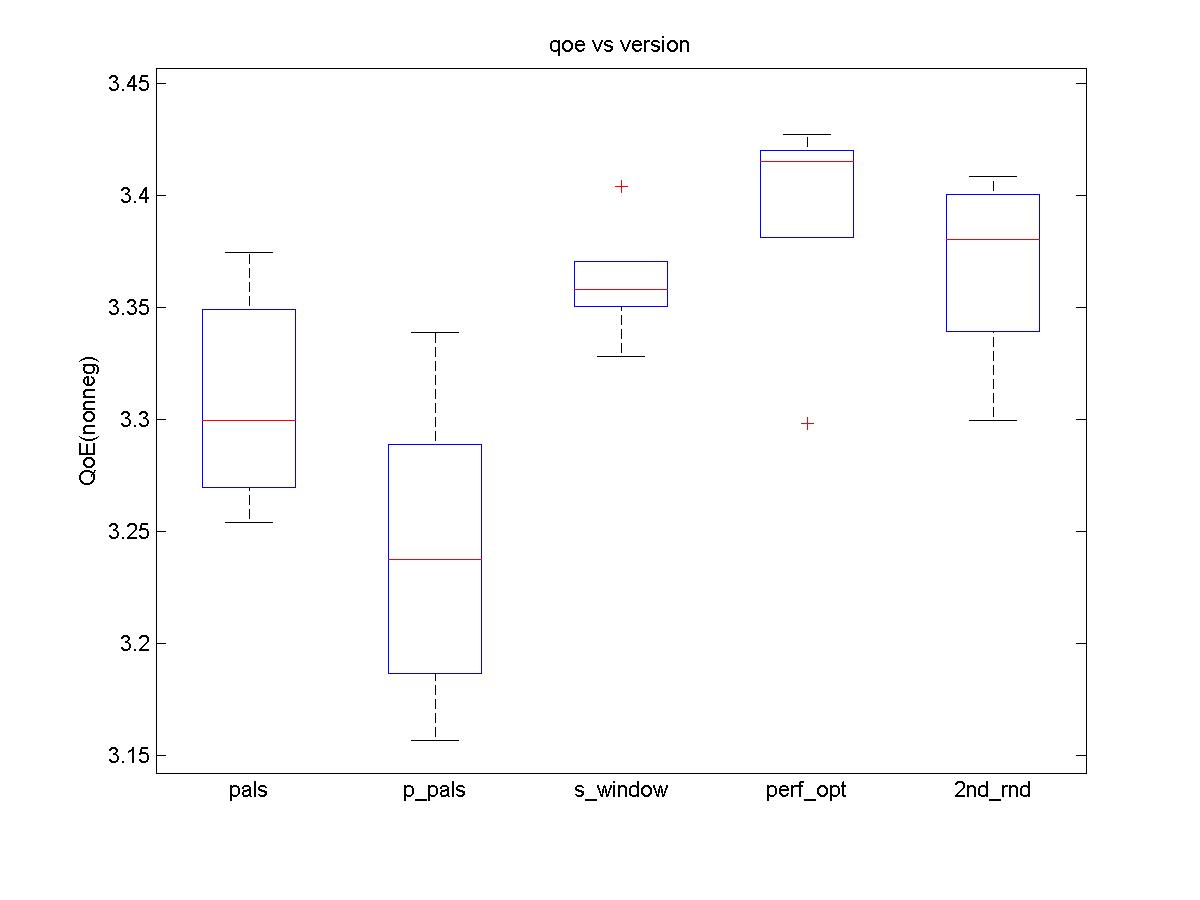
\includegraphics[width=0.45\textwidth]{../fig/con_qoe_version_part.jpg}
	}
	\subfigure[time]{
	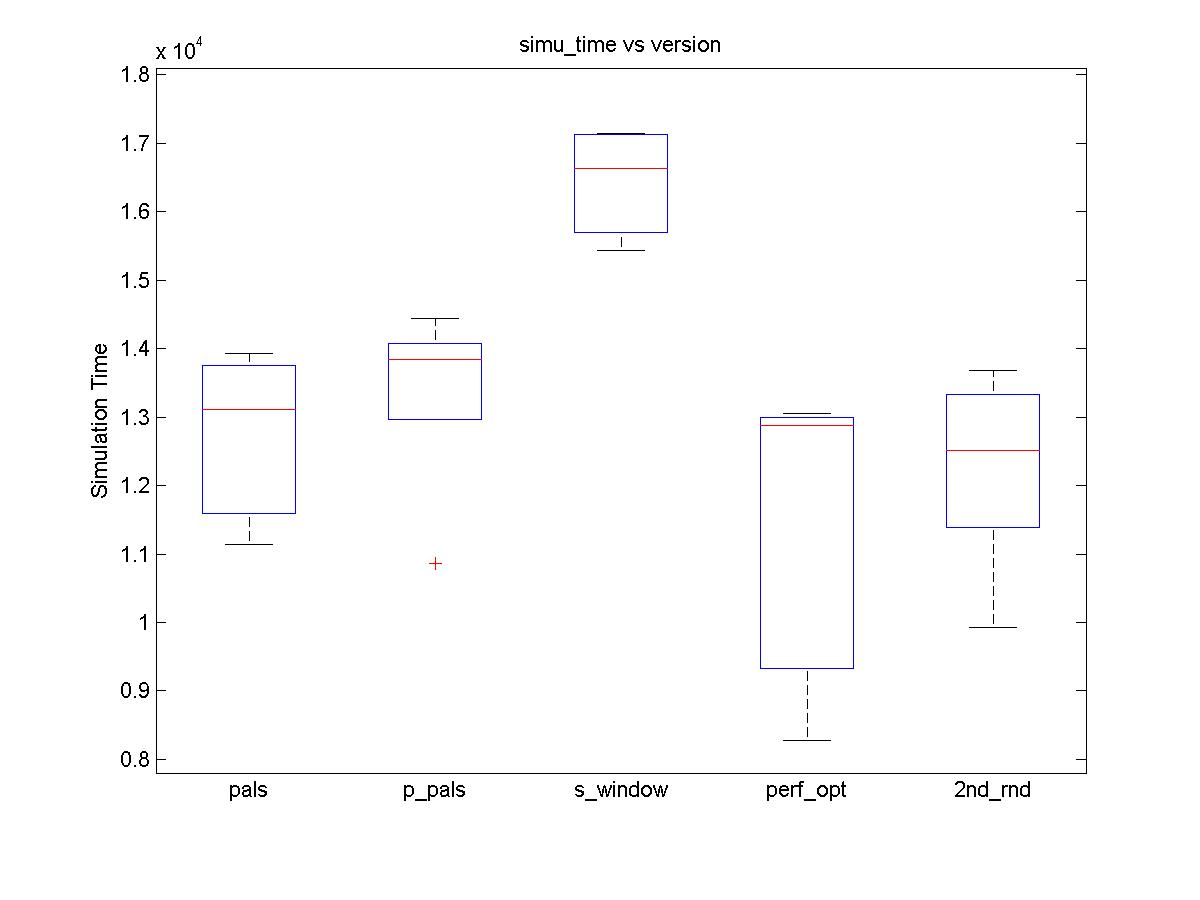
\includegraphics[width=0.45\textwidth]{../fig/con_time_version_part.jpg}
	}
	\caption{Conclusion, QoE and Performance}
\end{figure}
\end{frame}

\begin{frame}
\frametitle{Closing Remarks}
	\begin{itemize}
		\item Engineering approach v.s. academic approach:\\
		where is the biggest cake? 
		\item Time distribution:
			\begin{itemize}
				\item 70\%, literature survey.(30+ papers) 
				\item 15\%, bugfix of the platform, environment setup. 
				\item 5\%, first unified version(QoE:0.7$\rightarrow$3.3, 
				biggest improvement in this study)
				\item 10\%, scalable window, performance optimization, random 
				2nd section. (little outcome)
			\end{itemize}
	\end{itemize}
\end{frame}

\begin{frame}
\frametitle{Toolset}
\framesubtitle{find it on my homepage}
\begin{figure}
	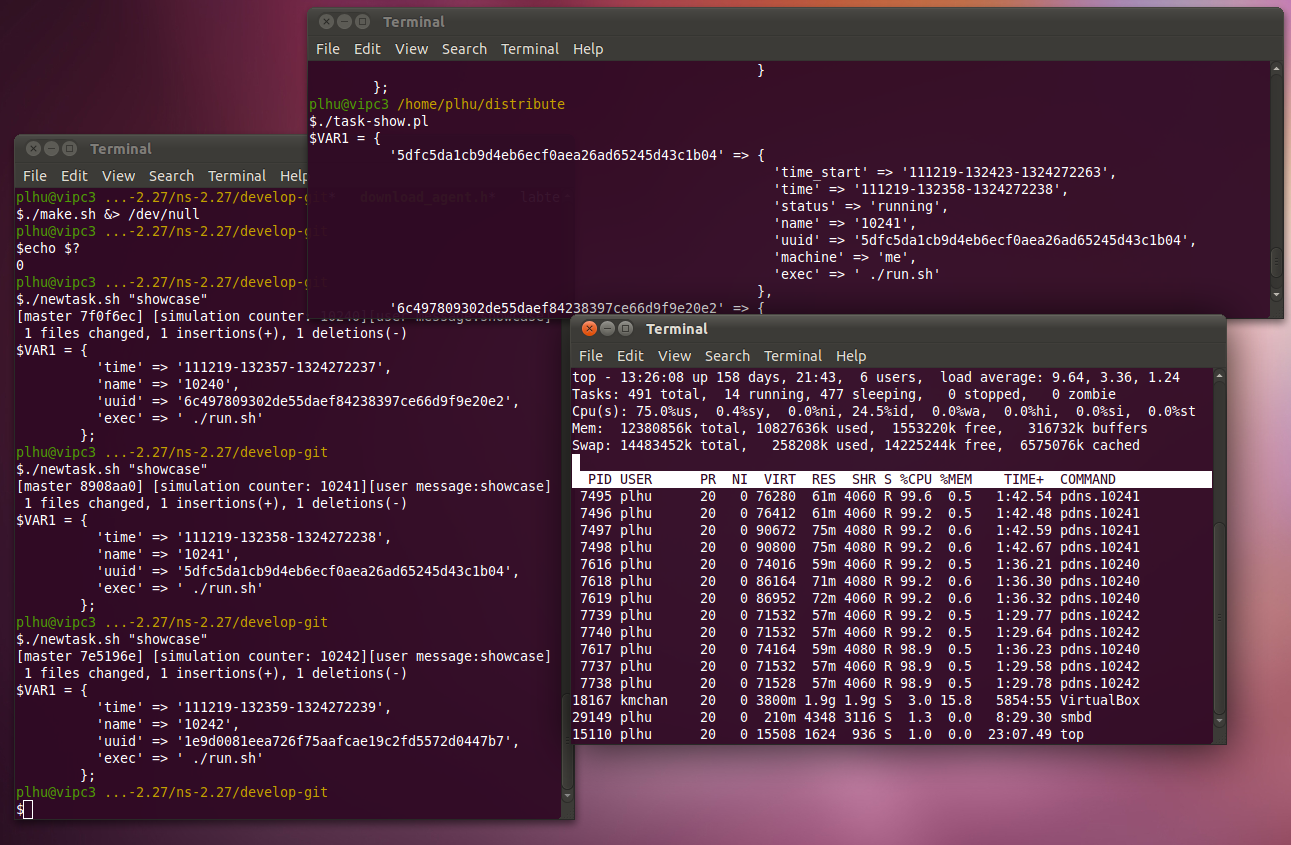
\includegraphics[width=0.85\textwidth]{../fig/distri_show.png}
	\caption{Lightweight Distributing Toolset }
\end{figure}
\end{frame}

\begin{frame}
\frametitle{Thanks}
\framesubtitle{some statistics}
Thanks! \\
Some statistics:
\begin{itemize}
	\item 6 big versions / 240 runs. 
	\item Auxilary Scripts:
	\begin{itemize}
	\item .sh:298 lines
	\item .pl:791  lines
	\item .m:133 lines
	\end{itemize}
	\item Simulation Code Difference:	
	\begin{itemize}
		\item download\_agent.cc: 1940 lines
		\item download\_agent.h: 301 lines
		\item labtesting.tcl: 84 lines
	\end{itemize}
\end{itemize}
\end{frame}

\end{document}